\chapter{Design}
The following chapter describes the design of the components required to implement the specified features from an architectural view. Each section represents one feature and illustrates which components will be developed. 

\begin{itemize}
	\item \textbf{Feature 1: Implement Transmission Chain}: Figure~\ref{fig:tx_chain_old} illustrates the current implementation of the transmission chain in \ac{AnSiAn}. This needs to be refactored and extended to a full transmission chain as illustrated in Figure~\ref{fig:tx_chain_new}.
	
	\item \textbf{Feature 2: RDS Transmission}: Figure~\ref{fig:rds_transmission} shows the required components for the RDS transmission feature. We need to be able to feed RDS data and audio into the modulator. Then we need to implement the construction of an RDS signal, which uses \ac{FM} for the audio and \ac{BPSK} for the additional information. As BPSK modulation is already implemented, this can be reused. Additionally we need to extend the UI to enable the user to define which RDS data should be transmitted. 
	
	\item \textbf{Feature 3: BPSK Demodulation improvements}: Figure~\ref{fig:bpsk_components} shows the context of the \ac{BPSK} Demodulation class which is used by \ac{RDS} and PSK31. This class should be refactored and improved.
	
	\item \textbf{Feature 4: Walkie-Talkie-Mode}: This feature consists of UI chan-ges and transmission changes. The UI should provide the functionality to select the Walkie-Talkie-Mode, listen to a specific frequency and enable/disable the transmission at any time. The transmission should then use the audio stream from the microphone, modulate it with a user-defined modulation scheme and transmit it using the HackRF. Figure~\ref{fig:walkie_talkie_components} depicts the components required for the transmission part. The UI changes are straightforward.
\end{itemize}


\begin{figure}
	\centering
	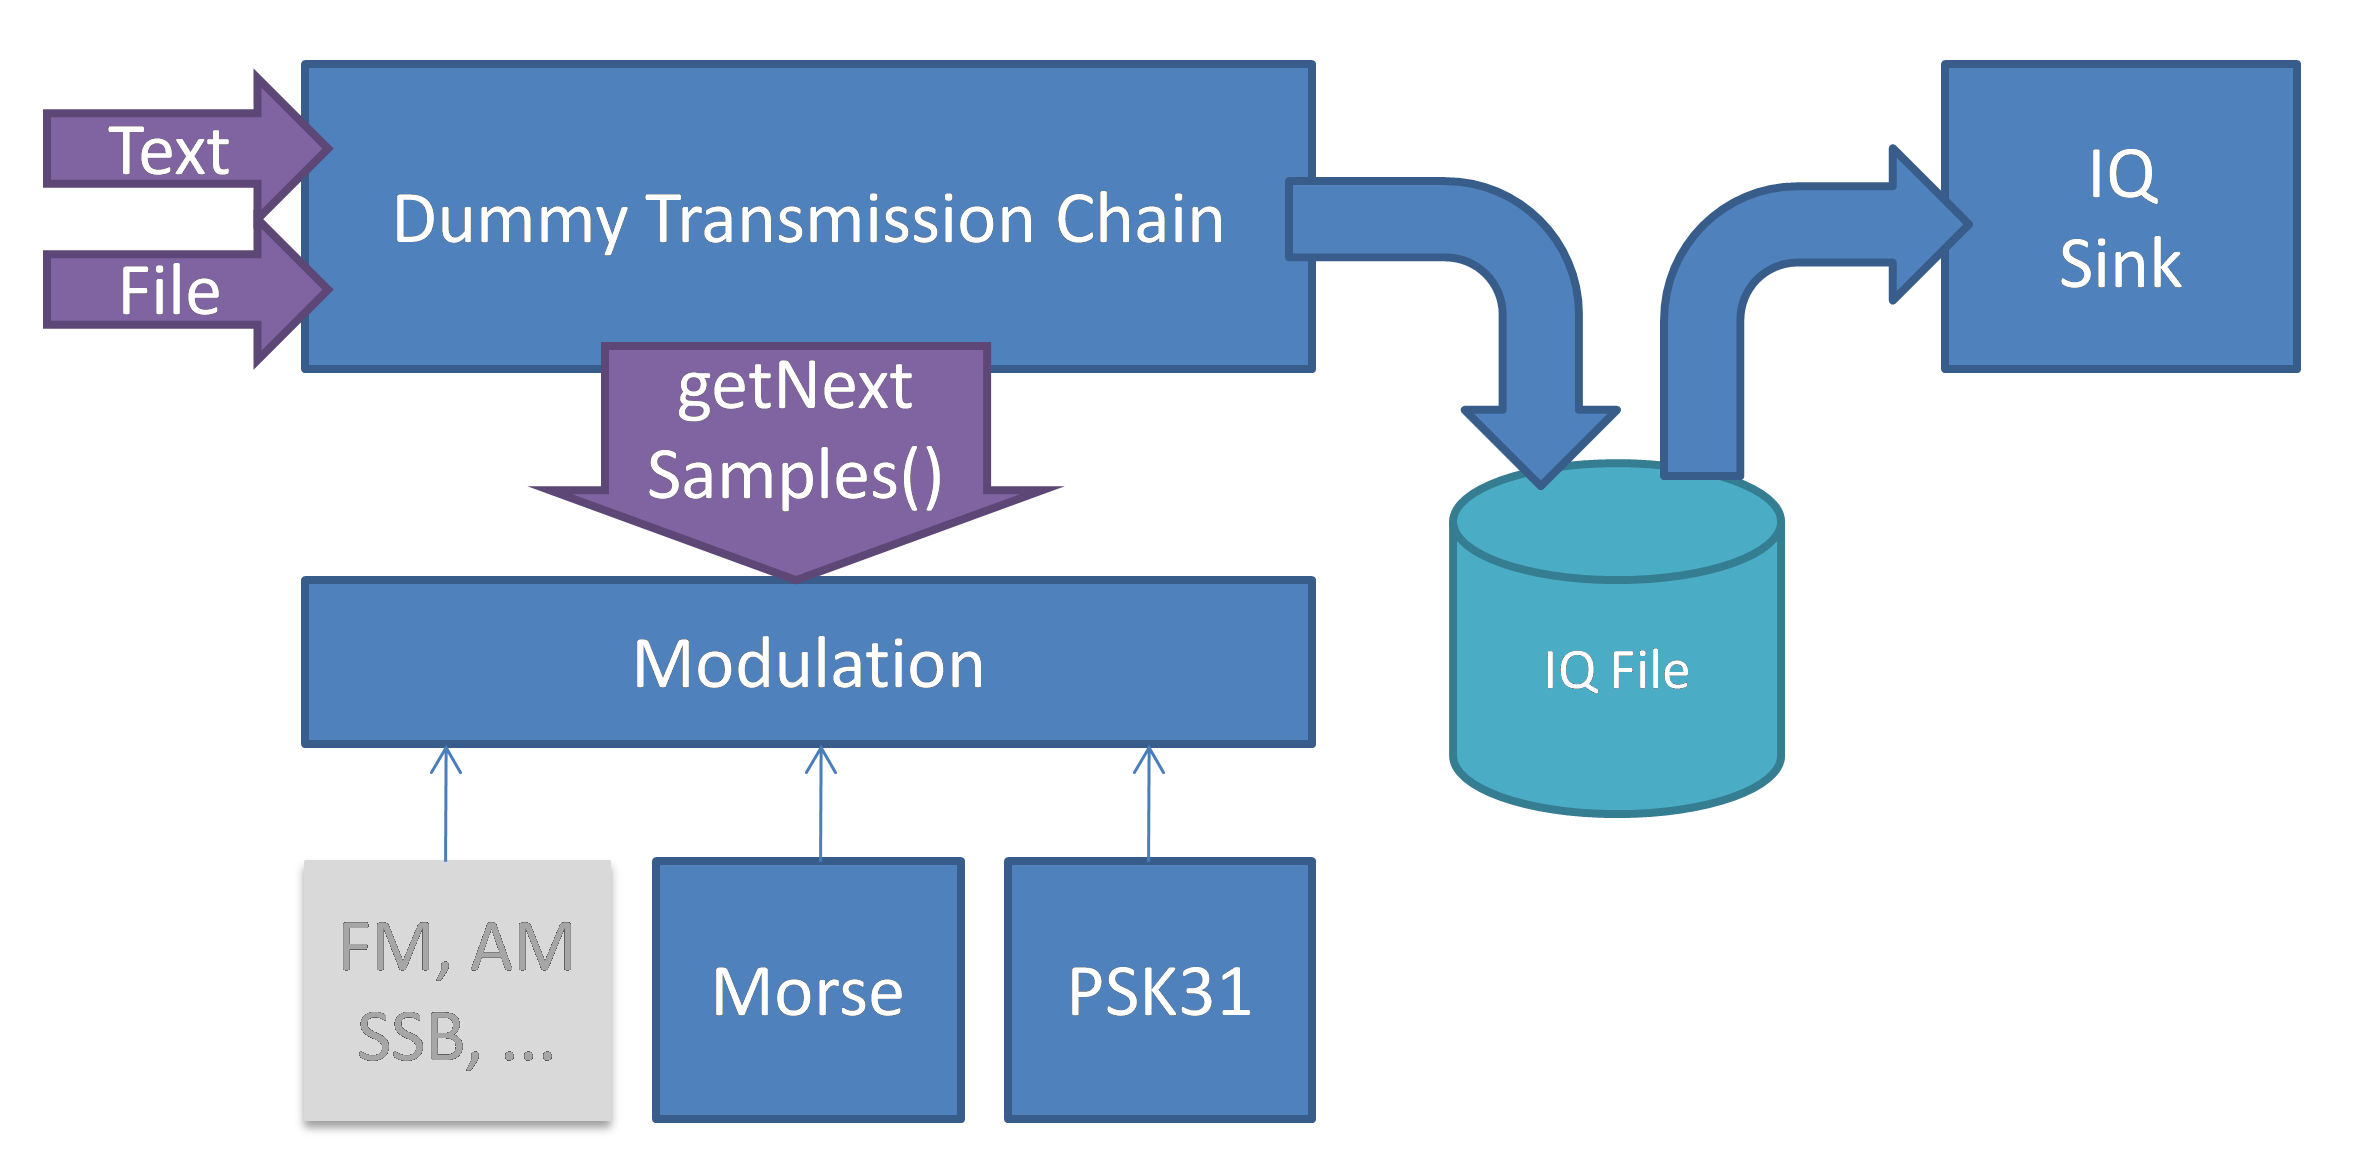
\includegraphics[width=1\linewidth]{gfx/TX_chain_step2.png}
	\caption{Transmission in current version of AnSiAn \cite{Mantz2016}}
	\label{fig:tx_chain_old}
\end{figure}

\begin{figure}
	\centering
	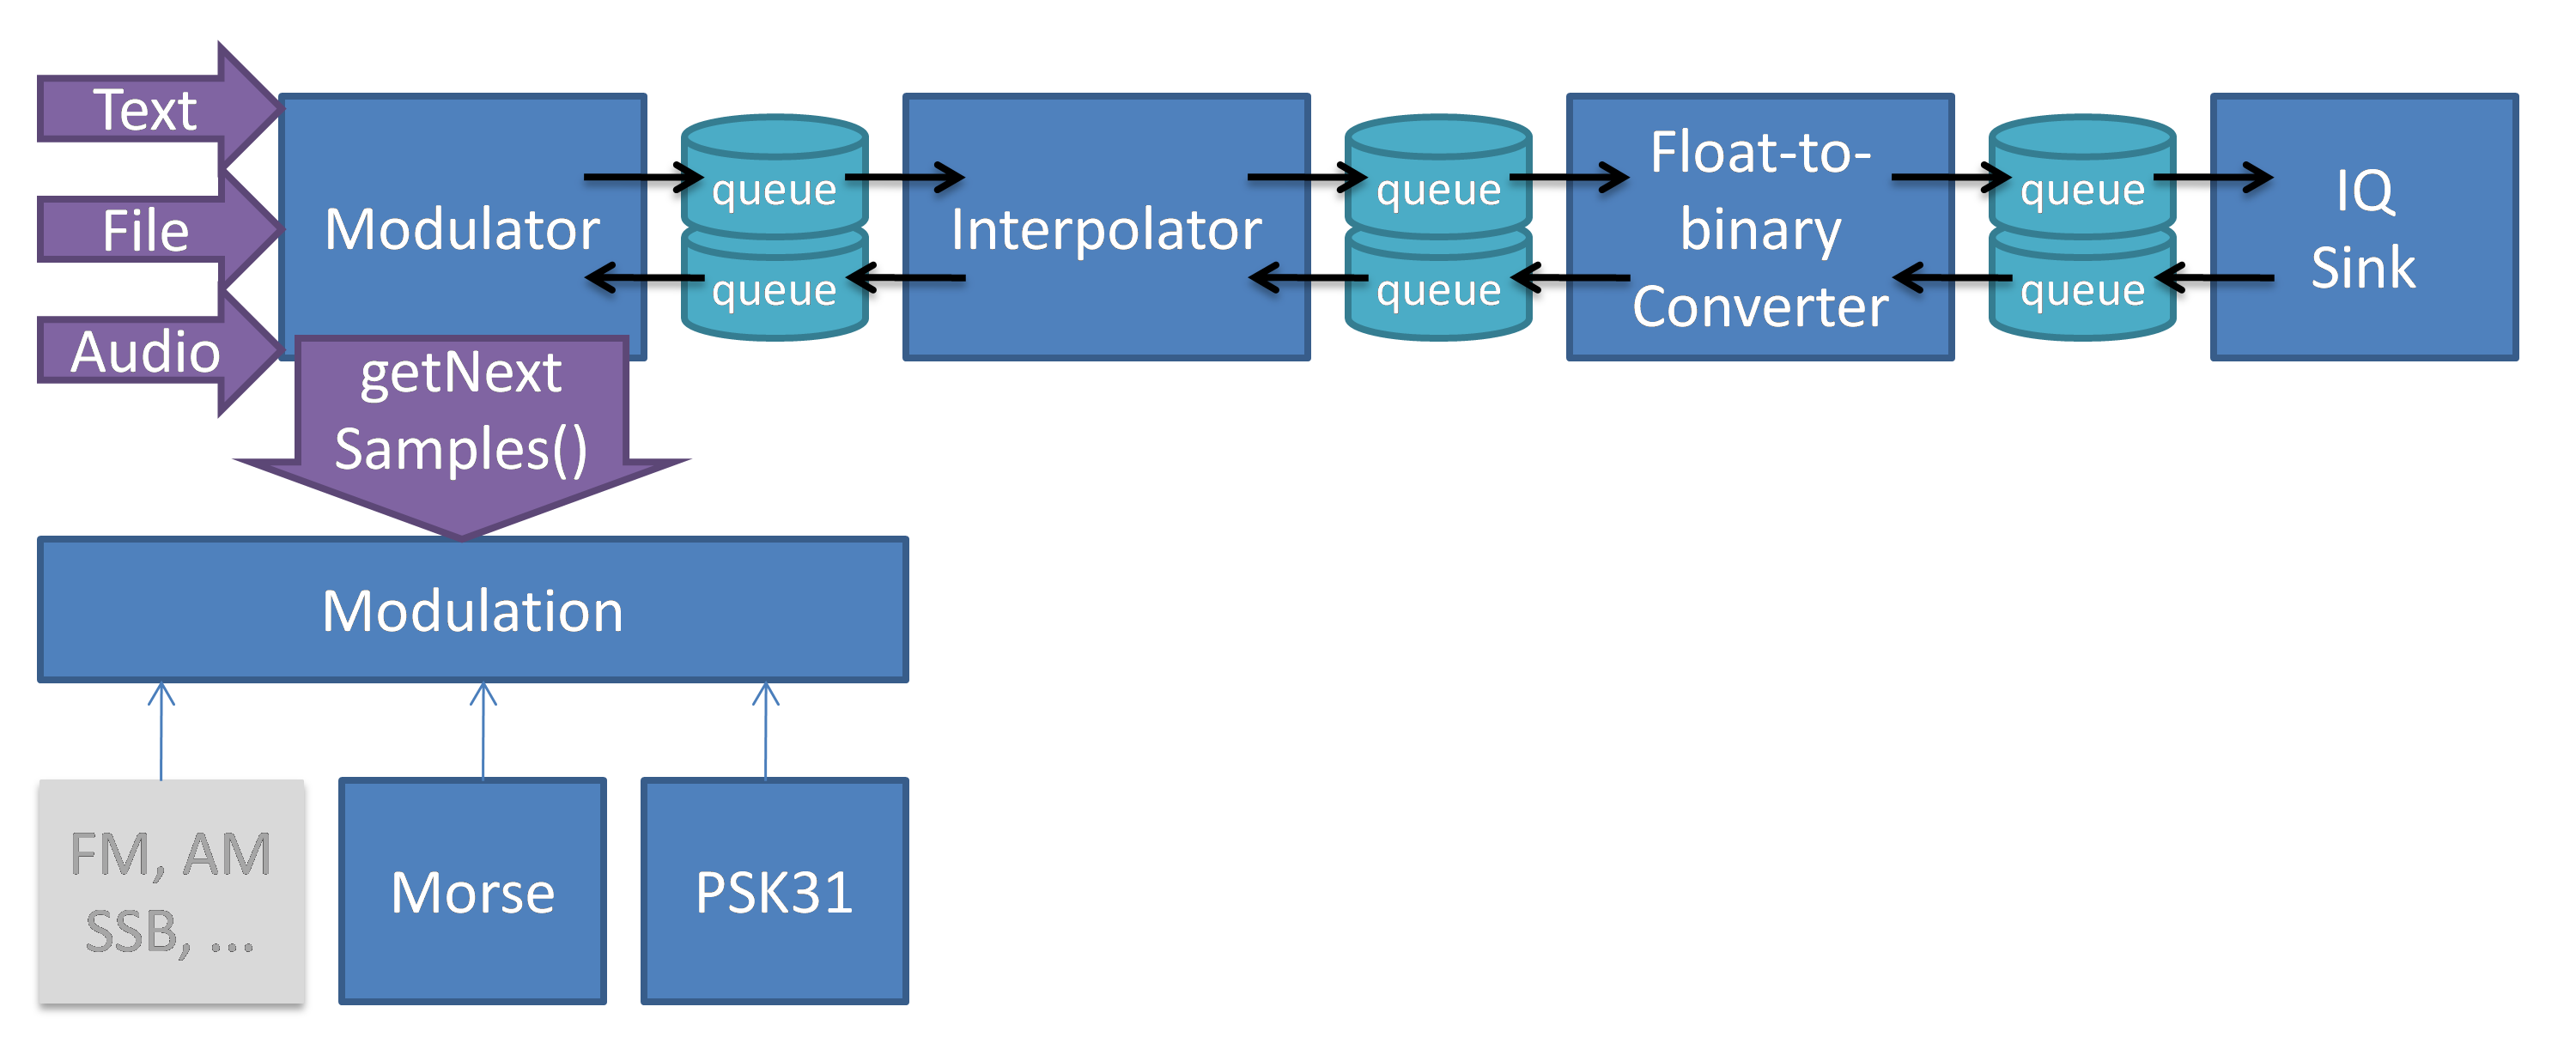
\includegraphics[width=1\linewidth]{gfx/TX_chain_final.png}
	\caption{Final transmission chain as suggested by \cite{Mantz2016}}
	\label{fig:tx_chain_new}
\end{figure}



\begin{figure}
	\centering
	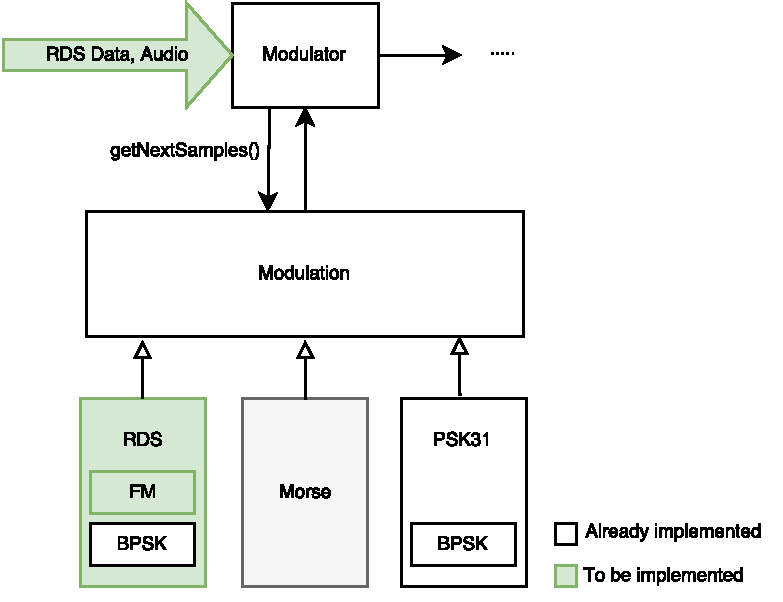
\includegraphics[width=1\linewidth]{gfx/feature2_components.pdf}
	\caption{Required Components for RDS Transmission}
	\label{fig:rds_transmission}
\end{figure}



\begin{figure}
	\centering
	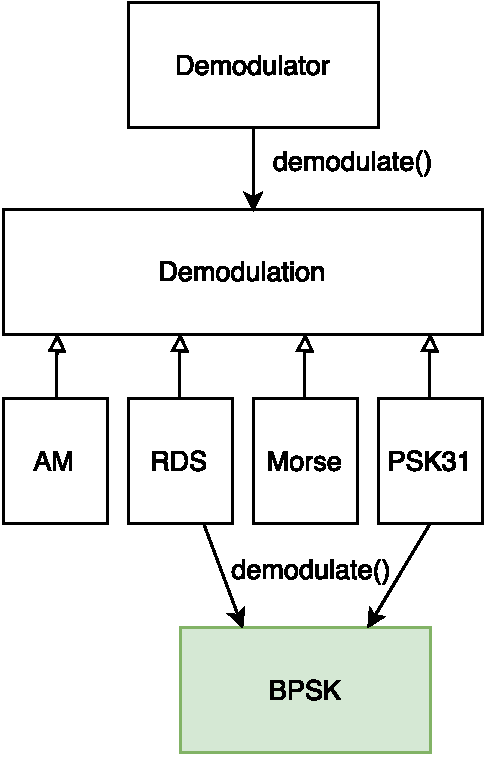
\includegraphics[width=0.5\linewidth]{gfx/feature3_components.pdf}
	\caption{Required Components for BPSK Demodulation Improvements}
	\label{fig:bpsk_components}
\end{figure}


\begin{figure}
	\centering
	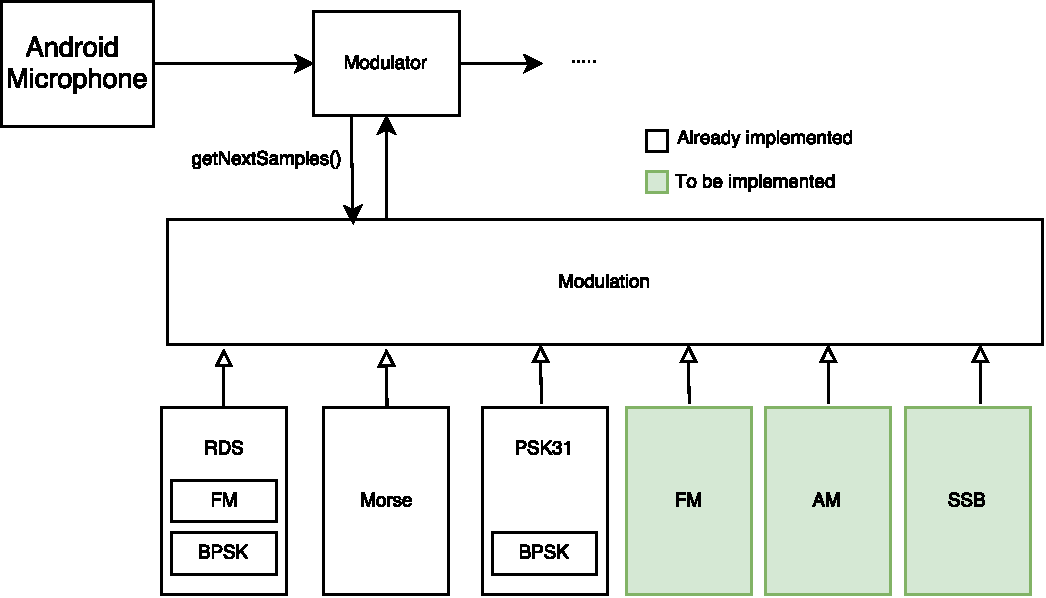
\includegraphics[width=1\linewidth]{gfx/feature4_components.pdf}
	\caption{Required Components for Walkie-Talkie-mode}
	\label{fig:walkie_talkie_components}
\end{figure}